\documentclass[ignorenonframetext,]{beamer}
\setbeamertemplate{caption}[numbered]
\setbeamertemplate{caption label separator}{: }
\setbeamercolor{caption name}{fg=normal text.fg}
\beamertemplatenavigationsymbolsempty
\usepackage{lmodern}
\usepackage{amssymb,amsmath}
\usepackage{ifxetex,ifluatex}
\usepackage{fixltx2e} % provides \textsubscript
\ifnum 0\ifxetex 1\fi\ifluatex 1\fi=0 % if pdftex
  \usepackage[T1]{fontenc}
  \usepackage[utf8]{inputenc}
\else % if luatex or xelatex
  \ifxetex
    \usepackage{mathspec}
  \else
    \usepackage{fontspec}
  \fi
  \defaultfontfeatures{Ligatures=TeX,Scale=MatchLowercase}
\fi
% use upquote if available, for straight quotes in verbatim environments
\IfFileExists{upquote.sty}{\usepackage{upquote}}{}
% use microtype if available
\IfFileExists{microtype.sty}{%
\usepackage{microtype}
\UseMicrotypeSet[protrusion]{basicmath} % disable protrusion for tt fonts
}{}
\newif\ifbibliography
\hypersetup{
            pdftitle={Deep Learning with Big Data: Alabama Highway Infrastructure},
            pdfauthor={Erik Johnson and Alexander Hainen},
            pdfborder={0 0 0},
            breaklinks=true}
\urlstyle{same}  % don't use monospace font for urls
\usepackage{graphicx,grffile}
\makeatletter
\def\maxwidth{\ifdim\Gin@nat@width>\linewidth\linewidth\else\Gin@nat@width\fi}
\def\maxheight{\ifdim\Gin@nat@height>\textheight0.8\textheight\else\Gin@nat@height\fi}
\makeatother
% Scale images if necessary, so that they will not overflow the page
% margins by default, and it is still possible to overwrite the defaults
% using explicit options in \includegraphics[width, height, ...]{}
\setkeys{Gin}{width=\maxwidth,height=\maxheight,keepaspectratio}

% Prevent slide breaks in the middle of a paragraph:
\widowpenalties 1 10000
\raggedbottom

\AtBeginPart{
  \let\insertpartnumber\relax
  \let\partname\relax
  \frame{\partpage}
}
\AtBeginSection{
  \ifbibliography
  \else
    \let\insertsectionnumber\relax
    \let\sectionname\relax
    \frame{\sectionpage}
  \fi
}
\AtBeginSubsection{
  \let\insertsubsectionnumber\relax
  \let\subsectionname\relax
  \frame{\subsectionpage}
}

\setlength{\parindent}{0pt}
\setlength{\parskip}{6pt plus 2pt minus 1pt}
\setlength{\emergencystretch}{3em}  % prevent overfull lines
\providecommand{\tightlist}{%
  \setlength{\itemsep}{0pt}\setlength{\parskip}{0pt}}
\setcounter{secnumdepth}{0}

\title{Deep Learning with Big Data: \newline Alabama Highway Infrastructure}
\author{Erik Johnson and Alexander Hainen}
\date{04 December, 2017}

\begin{document}
\frame{\titlepage}

\begin{frame}{}

\includegraphics{/home/ebjohnson5/Dropbox/pkg.data/alabama_roads/raw/training_data/guardrail/22guardrail.jpg}

\end{frame}

\begin{frame}{}

\includegraphics{/home/ebjohnson5/Dropbox/pkg.data/alabama_roads/raw/training_data/signals/09signals.jpg}

\end{frame}

\begin{frame}{What is big data?}

\begin{itemize}
\tightlist
\item
  Images and Video are big data

  \begin{enumerate}
  \def\labelenumi{\arabic{enumi}.}
  \tightlist
  \item
    Need to explore quickly and accurately
  \item
    Possible efficiency gains (better questions, better answers)
  \item
    In globally competitive environment huge gains to first movers.
  \end{enumerate}
\item
  Big data source examples:

  \begin{enumerate}
  \def\labelenumi{\arabic{enumi}.}
  \tightlist
  \item
    Google Streetview: Road infrastructure detection (guardrails,
    traffic lights, rumble strips, lane information)
  \item
    Drones: Storm Damage assessment (tree mapping, structure changes,
    power line status)
  \item
    Traffic cameras: Traffic congestion and accident identification from
    traffic cameras.
  \item
    Crowdsourced instagram photos, etc.
  \end{enumerate}
\end{itemize}

\end{frame}

\begin{frame}{Big data challenges:}

\begin{itemize}
\tightlist
\item
  Costly to understand the meaning and information in the pictures.

  \begin{enumerate}
  \def\labelenumi{\arabic{enumi}.}
  \tightlist
  \item
    How to classify? (students/employees, etc.)
  \item
    Prone to human error and missing information.
  \item
    If new category is added must go back and reclassify all previous
    images.
  \item
    Need real time abilities (24 hours/day 7 days/week)
  \end{enumerate}
\item
  Solution:

  \begin{enumerate}
  \def\labelenumi{\arabic{enumi}.}
  \tightlist
  \item
    Automate using rapidly advancing deep learning algorithms.
  \end{enumerate}
\end{itemize}

\end{frame}

\begin{frame}{Application}

This application focuses on using big data and deep learning to cheaply
and efficiently classify infrastructure on Alabama highway 82 between
Tuscaloosa and Montgomery.

This process will illustrate the following:

\begin{enumerate}
\def\labelenumi{\arabic{enumi}.}
\tightlist
\item
  How to build a big data set using free/low-cost data

  \begin{itemize}
  \tightlist
  \item
    Publicly available road shapefiles.
  \item
    Google Streetview images
  \end{itemize}
\item
  How to train and classify images using free and simple algorithms

  \begin{itemize}
  \tightlist
  \item
    Google Tensorflow
  \item
    Inception v3 algorithm and retraining
  \end{itemize}
\end{enumerate}

\end{frame}

\begin{frame}[fragile]{Start with any freely available road shapefile.}

\begin{verbatim}
* Here, we use Alabama Highway 82 
\end{verbatim}

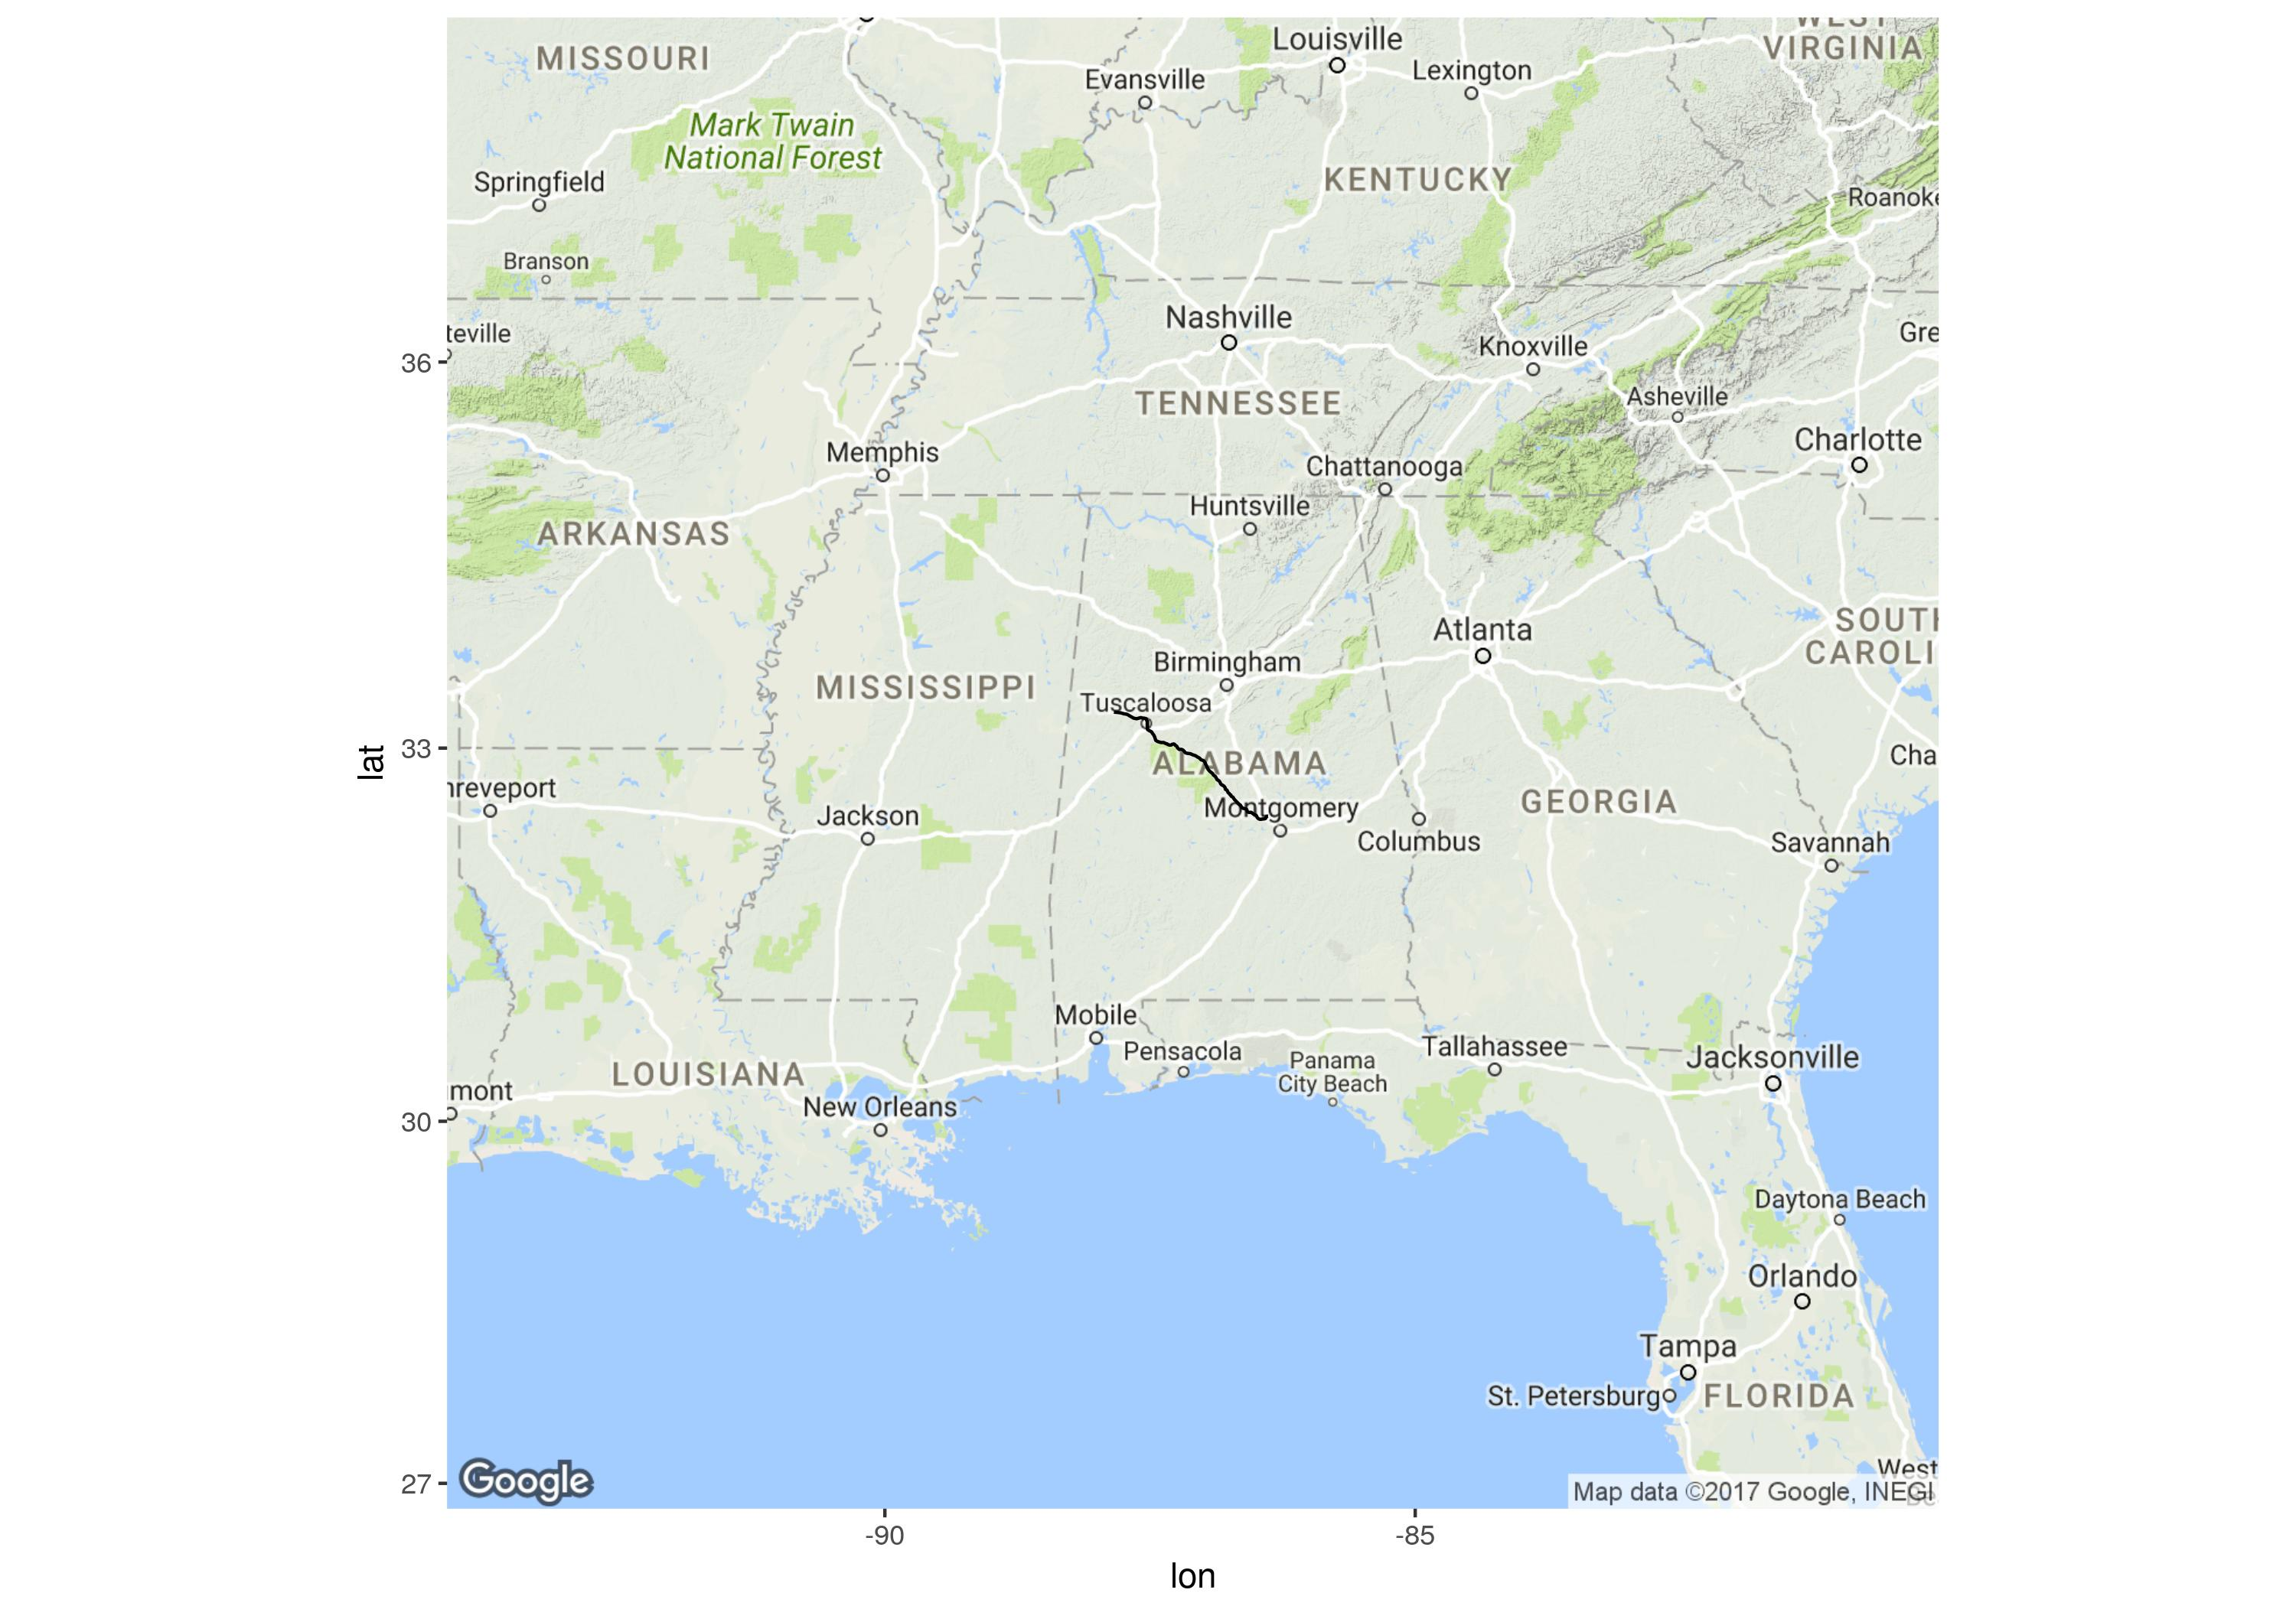
\includegraphics[width=300px]{Images/highway}

\end{frame}

\begin{frame}{Find all google streetview snapshots locations}

\begin{itemize}
\tightlist
\item
  A bit of coding, processing, and downloading streetview metadata to
  aim the cameras, set the zoom levels.
\item
  There are 20104 camera locations with a rear and forward camerabearing
  set for each.
\item
  Here are the first 6.
\end{itemize}

\begin{table}[H]
\centering\begingroup\fontsize{6}{8}\selectfont

\begin{tabular}{l|l|r|r|r|r|r}
\hline
snap\_date & pano\_id & order & lat & lng & bear.lead & bear.lag\\
\hline
2016-05 & lk4vKW941erchBtIeRqenA & 2 & 33.28436 & -87.84009 & 92.64210 & -87.35684\\
\hline
2016-05 & 8sR6h5ILqzn3NSvXhYhP\_g & 3 & 33.28435 & -87.84000 & 100.73244 & -87.35785\\
\hline
2016-05 & 5YeX5au5BuKvr-VE8mnHYg & 4 & 33.28434 & -87.83991 & 98.83936 & -79.26751\\
\hline
2016-05 & 7ixd4IHZEO1aUZSMVo\_OcQ & 5 & 33.28433 & -87.83982 & 97.23829 & -81.16059\\
\hline
2016-05 & LMB6s5\_qe2463PujYfHafw & 6 & 33.28432 & -87.83973 & 97.02418 & -82.76167\\
\hline
2016-05 & 6TTjtyYJ1NmTOpE0T-\_Yzg & 7 & 33.28431 & -87.83964 & 96.80426 & -82.97577\\
\hline
\end{tabular}\endgroup{}
\end{table}

\end{frame}

\begin{frame}{Take Google Streetview snapshots}

\begin{itemize}
\tightlist
\item
  We then feed the location and variable parameters to the google
  streetview api and download all 40208 pictures.
\end{itemize}

\includegraphics{/home/ebjohnson5/Dropbox/pkg.data/alabama_roads/raw/training_data/guardrail/22guardrail.jpg}

\end{frame}

\begin{frame}{}

\includegraphics{/home/ebjohnson5/Dropbox/pkg.data/alabama_roads/raw/training_data/signals/09signals.jpg}

\end{frame}

\begin{frame}{Human Classification of streetview photos}

\begin{itemize}
\tightlist
\item
  To start the classification we must teach the machine to recognize
  different features.
\item
  Human selects 30-50 photos for each class.
\end{itemize}

\begin{enumerate}
\def\labelenumi{\arabic{enumi}.}
\tightlist
\item
  30 photos from streetview downloads with guardrails
\item
  30 photos from streetview downloads with traffic lights
\item
  30 photos from streetview downloads with rumble strips
\end{enumerate}

\begin{itemize}
\tightlist
\item
  Each set of photos is put into its own folder (guardrail, etc.)
\end{itemize}

\end{frame}

\begin{frame}{Training machine to recognize classes}

\begin{itemize}
\tightlist
\item
  We use transfer learning on google's Inception v3 algorithm for this
  demonstrations
\item
  Inception v3 is a deep learning machine that takes a long, long, time
  to build a model
\item
  We retrain the last step to recognize the guardrails, traffic lights,
  rumble strips, etc.
\end{itemize}

Best analogy: Inception v3 is a toddler. We do not want to waste time
and resources raising a toddler. We just want to teach a toddler to
recognize a set of new objects such as a spoon. Show the toddler 30
spoons and they gain the ability to classify spoon objects.

\end{frame}

\begin{frame}{Training Diagnostics}

\begin{itemize}
\tightlist
\item
  Training diagnostics through tensorboard.
\end{itemize}

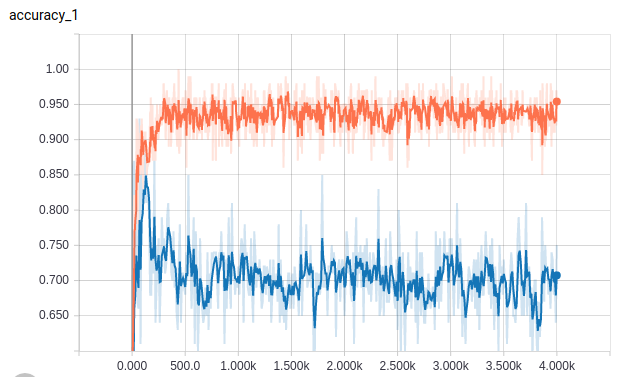
\includegraphics[width=300px]{Images/tensorTraining}

\end{frame}

\begin{frame}{Classify all photos}

\begin{itemize}
\tightlist
\item
  The next step is to classify how each of the 40207 photos using the
  trained model.
\item
  The overall probability of all classes sum to 1 for each photo.
\end{itemize}

\[ \sum_{classes} Pr(class_i) = 1\]

\end{frame}

\begin{frame}{Classification: Rumble Strips only}

\begin{center}\includegraphics[width=200px]{/home/ebjohnson5/Dropbox/pkg.data/alabama_roads/raw/snapshots/pano_id:zZ39CumiCqaxS9-1n6erDg_lead} \end{center}

\begin{table}[H]
\centering\begingroup\fontsize{6}{8}\selectfont

\begin{tabular}{l|l|r}
\hline
fName & category & score\\
\hline
pano\_id:zZ39CumiCqaxS9-1n6erDg\_lead.jpg & rumble & 0.95842\\
\hline
pano\_id:zZ39CumiCqaxS9-1n6erDg\_lead.jpg & guardrail & 0.04124\\
\hline
pano\_id:zZ39CumiCqaxS9-1n6erDg\_lead.jpg & signals & 0.00033\\
\hline
\end{tabular}\endgroup{}
\end{table}

\end{frame}

\begin{frame}{Classification: Traffic Signal only}

\begin{center}\includegraphics[width=200px]{/home/ebjohnson5/Dropbox/pkg.data/alabama_roads/raw/snapshots/pano_id:-km7JQTMeLsO9k7uF_cnsg_lag} \end{center}

\begin{table}[H]
\centering\begingroup\fontsize{6}{8}\selectfont

\begin{tabular}{l|l|r}
\hline
fName & category & score\\
\hline
pano\_id:-km7JQTMeLsO9k7uF\_cnsg\_lag.jpg & signals & 0.99850\\
\hline
pano\_id:-km7JQTMeLsO9k7uF\_cnsg\_lag.jpg & guardrail & 0.00149\\
\hline
pano\_id:-km7JQTMeLsO9k7uF\_cnsg\_lag.jpg & rumble & 0.00001\\
\hline
\end{tabular}\endgroup{}
\end{table}

\end{frame}

\begin{frame}{Classification: Rumble Strips and Guardrail}

\begin{center}\includegraphics[width=200px]{/home/ebjohnson5/Dropbox/pkg.data/alabama_roads/raw/snapshots/pano_id:zZq1fNpgOGCGAWylAjnidw_lag} \end{center}

\begin{table}[H]
\centering\begingroup\fontsize{6}{8}\selectfont

\begin{tabular}{l|l|r}
\hline
fName & category & score\\
\hline
pano\_id:zZq1fNpgOGCGAWylAjnidw\_lag.jpg & rumble & 0.54766\\
\hline
pano\_id:zZq1fNpgOGCGAWylAjnidw\_lag.jpg & guardrail & 0.45233\\
\hline
pano\_id:zZq1fNpgOGCGAWylAjnidw\_lag.jpg & signals & 0.00001\\
\hline
\end{tabular}\endgroup{}
\end{table}

\end{frame}

\begin{frame}{Results:}

Classified images from this example project can be used in a variety of
ways:

\begin{enumerate}
\def\labelenumi{\arabic{enumi}.}
\tightlist
\item
  Highway infrastructure inventory accounting.
\item
  Interactive mapping.
\end{enumerate}

\end{frame}

\end{document}
